\documentclass[12pt,a4paper]{article}
\usepackage{ucs}
\usepackage{caption}
\usepackage[latin1,utf8x]{inputenc}
\usepackage{amsmath}
\usepackage{caption}
\captionsetup{font=small,labelfont=bf}
\usepackage[danish]{babel}
\usepackage[rmargin=3cm,tmargin=3.3cm]{geometry}
\usepackage{listings}
\usepackage{color}
\setlength{\parindent}{0pt}
\setlength{\parskip}{1ex plus 0.5ex minus 0.2ex}
\usepackage{graphicx}
\usepackage{fixltx2e}

\usepackage[T1]{fontenc}
\usepackage{textcomp}


%insert links
\usepackage{hyperref}
\usepackage{fancyhdr,lastpage}	
\pagestyle{fancy}


\definecolor{mygreen}{rgb}{0,0.6,0}
\definecolor{myblue}{rgb}{0,0,1}
\definecolor{myyellow}{rgb}{0.7,0.7,0}
\definecolor{myblack}{rgb}{0,0,0}

\lstset{
	basicstyle=\ttfamily\footnotesize
	breaklines=true,
	numbers=left, 
	commentstyle=\color{mygreen},
	stringstyle=\color{myyellow},
}

%header
\lhead{ 
	Embedded Systems A2\\
	02131 \\ 
}
\chead{ 
}
\rhead{ 11 November, 2013 \\ \bigskip  }

%Footer
\lfoot{
	\rule{\textwidth}{0.1mm}\\
}

\cfoot{}
\rfoot{\ \\ \scriptsize{Side \thepage\ af \pageref{LastPage}}}

\begin{document}

%Forside
\begin{titlepage}
	\begin{center}
		\vspace*{13\baselineskip}
		\huge
		\bfseries
		Embedded Systems\\ 
		\ \\
		02131 \\[5\baselineskip]

		\normalfont
		\Large
		R-peak detection. \\
		Assignment 2\\	
		2013

		\small
		\vfill
	\end{center}	
	\begin{flushleft}
		Jakob Welner, s124305\\
	 	Jacob Gjerstrup, s113440\\
	\end{flushleft}
\end{titlepage}

\ \\
\section*{Abstract}
The task of this assignment was to show by proof-of-concept that a dedicated processor could be created through the Gezel hardware description language. This dedicated processor was created in such a way that it could accept instructions in the form of assembly commands, enabling it to execute the Moving Window Integration filter from Assignment 1. The dedicated processor was then attached to a bus, which again was attached to an external memory module where the data samples were located. A protocol for communicating with the bus and memory module was then implemented.

\thispagestyle{empty} 
\newpage

%Table of Contents
\tableofcontents
\thispagestyle{empty} 
\newpage

%Reset pagecount
\setcounter{page}{1}

%Alm. sider
\ \\
\section{Introduction}
	After successfully proving in Assignment 1 that the QRS algorithm could be implemented in software, Medembed now wants a proof of concept that the algorithm can be optimized further by implementing the most demanding parts of it in hardware. From Assignment 1 it was found that the Moving Window Implementation was taking up the most processing power so it was decided to implement that. Using a Hardware Description Language (HDL) called Gezel, the filter can be implemented on simulated hardware, thus making it obvious whether such implementation can serve the requirements.
	This report will discuss how the filter will be implemented through Gezel, as well as going more in depth on the topics: Modules of the CPU, Instruction set for the CPU, Integration of the CPU into a combined system, and finally, the critical parts of the CPU, i.e. speed, power consumption and size.\\
	For the purpose of this report, the data for the filter will be loaded through a file one data point at a time and then processed by the simulated hardware.\\
	
\subsection{Requirements}
Below follows a list of functional and non-functional requirements:\\

\textbf{ Functional requirements for the application:}
\begin{itemize}
	\item Each module of the processor must first be built, run and tested by their own
	\item An instruction set must be designed
	\item A CPU that can execute the instructions must be designed
	\item The CPU must be integrated into a larger system
	\item The value of the system must be analysed in terms of size, speed and power

\end{itemize}
\textbf{Non-functional requirements for the application:}
\begin {itemize}
	\item The system must be implemented with the use of Gezel
\end{itemize}

\section{Analysis}
 	In order to initiate the structure- and design-process of the program, a number of questions needed to be answered first:\\
 	
 	\begin{enumerate}
	\item How could the C-code be compiled into hardware instructions
	\item Which instructions would be needed to accomplish this?
	\item Which hardware modules would be needed to execute the instructions?	
	\item How could the CPU be designed in order to understand the instruction set?
	\item How could the CPU be integrated into a system?
	\item What would the critical parts of the system be and how could these be analysed?
\end{enumerate}

\subsection{Problem 1: Hardware modules}
	To gain a basic understanding of GEZEL and hardware design, an initial guide was given that suggested the creation of the following modules, as well as how to make these: Counter, Adder, Multiplexer, Arithmetic Logic Unit (ALU) with and without status flags, a register file and an instruction memory block. The main concern here was to understand the difference between software and hardware design.\\
	
\subsection{Problem 2: Instruction set}
	Designing the instruction set was a fairly arbitrary task, as there were very few limitations and the instructions in theory could be anything. The first question here was whether the instructions should be able to execute on single cycles or be more complex and execute across several cycles (RISC vs. CISC).\\
	The second question was how to ensure that these instructions could actually be interpreted by the processor, and what actual instructions needed to be there.\\
	\\
	
\subsection{Problem 3: Implementation of the CPU}
	Once the instruction set was finished, the next part would be to implement a CPU that could understand and execute the instruction set. To do this, a block diagram was to be designed to get an overview of how each component should be connected, but the design of this diagram would depend entirely on the instructions needed.\\
	Once the block diagram was completed and all components were connected, the next issue became to distinguish control- and data signals - here, control signals configure a single component whereas data signals carry data between the components.\\
	Finally, the last question was how to combine the buildingblocks from before into a functional CPU.\\
	
\subsection{Problem 4: System Integration}
	Having a functional CPU, the next step was to integrate it into a premade platform consisting of a bus and an external memory. To do this, the CPU needed to be able to communicate and react properly to the bus. The bus uses a master/slave protocol where the CPU is the master and the external memory the slave. The protocol between the master and the slave was predefined and functional in the provided Platform, 
	so the main objective was to implement the correct logic that would allow the master to send data to the slave, wait for a return signal as well as receive and save the returned data.\\
	
\subsection{Problem 5: Critical parts}
	There are three terms that needs to be discussed when it comes to the critical parts of a system: Size, speed and power.\\
	The speed of a dedicated system is the most important of these up to the point where you are certain that it is capable of making the maximum needed computations within the allowed time frame. In the case of this assignment it is a matter of handling 250 data points per second and display the result to the user. However, once this has been achieved, a further increase in speed will generally mean raising the unit cost as well as potential power consumption.\\
	Power and size are equally important, as the bigger the processor is, the more cumbersome the ECG scanner will be for a user to wear, and the more power it consumes, the more often it will need to be recharged or have the battery replaced. Therefore, the three problems becomes:
	
	\begin{itemize}
		\item Is the CPU fast enough and where is it mainly spending the time?
		\item Which modules are taking up space on the chip and what can be done to reduce this?
		\item How much energy does the system consume and what can be done to reduce that?
	\end{itemize}
	
\section{Implementation}
\subsection{Hardware modules}
	To build the initial modules, it was decided that each module should have a testbench associated in order to validate their functionality before progressing. The code for these modules as well as their testbenches can be seen in the appendix.\\
	The modules were then treated as basic building blocks for the CPU.\\
	
\subsection{Instruction set}
	For this report, RISC was chosen as a basis for the instruction set. A theoretical assembly code was made based on the assumption of single-clock instructions, where instructions were added to the list as they became needed. From this theoretical assembly code the instruction set was extracted.\\
	\\
	To ensure the CPU could access and understand this instruction set, the instructions needed a certain format. From using Gezel for the development along with implementing the instruction memory using an ipblock in Gezel, the instructions needed to be listed in a file and formatted as hexadecimal numbers, each command having a unique address and the actual command separated by a space. The commands were put in a file called program.txt, which would allow the ipblock in Gezel to open it and access the different addresses similar to an actual memory block.
	While implementing the different instructions it turned out that changing hex numbers, knowing what is where and testing individual cases proved difficult. For this reason an actual assembler was written in Python, which would take the assembler commands and write out the program.txt file in a format that Gezel would then understand. This sped up the development significantly, reduced human error as well as made it possible to program the CPU directly by assembly commands.
	To produce the instruction set, the initial task was to replicate the behaviour of the C-code from assignment 1. However, it turned out that when considering the previous C-implementation in terms of hardware execution, much could be done to optimize it. While the initial C-implementation was summing the past 30 values for each new datasample, dividing each value with 30, it was obvious that there was much to be done.
	Firstly, based on new insight into hardware arithmetic it is clear that division is a much more complex operation than adding and subtracting, hence, it is beneficial to reduce number of divisions to a minimum. This meant that dividing the sum by 30 instead of dividing each value by 30 and then summing, would improve the performance significantly. Furthermore, accessing memory from hardware is much slower than handling registers so that reading 30 values for each new sample wasn't ideal either. Instead the sum was implemented as an accumulator, which would maintain the sum of the past 30 value across clock-cycles and only subtract the oldest value as well as adding the latest value, thus moving the sum instead of redoing it. Changing the implementation like so would cut down memory access from 30 to 2 for each sample as well as cut down divisions from 30 to 1 pr. sample. 
	Division however, proved a completely different challenge. Implementing division in hardware within few clock-cycles is by no means trivial. It was found that for this particular case, the exact numbers did not matter as much as the difference between each sample, which is the only factor when finding peaks. Similarly, for measuring heartbeat intensity it was concluded that the value is arbitrary in either case. Finally, in the case of this particular assignment, all values used are integers, meaning that they are rounded off and not necessarily precise to begin with. For these reasons the decision for implementing division by 30 was instead to approximate it.
	Given that multiplication is much simpler to implement than division and that bitshifting is close to free, a python script (See appendix) was made to calculate the best approximation to $1/30$ by combining multiplication and bitshifting, while staying within 32-bit values.
	It was found that a reasonable approximation could be made by multiplying by $4369$ and bitshifting right by $17$. With this in mind, the instruction set could be made, which ended up consisting of 11 separate instructions:\\
	
	\begin{itemize}
			
			\item LOAD R0 X: \qquad[$R0=mem(X)$]
			\item STRE X R0: \;\qquad[$mem(X)=R0$]
			\item MOVE R0 R1: \,\,\quad[$R0=R1$]
			\item ADD R0 R1 R2: \quad[$R0=R1+R2$]
			\item SUB R0 R1 R2: \quad[$R0=R1-R2$]
			\item ADDI R0 R1 X: \quad[$R0=R1+X$]
			\item SUBI R0 R1 X: \quad[$R0=R1-X$]
			\item SHRI R0 R1 X: \quad[$R0=R1>>X$]
			\item MULI R0 R1 R2: \quad[$R0=R1*R2$]
			\item BLILT R0 R1 X: \quad[$if\;(R0>R1)\;goto\;X$]
			\item BRCH X: \qquad\qquad[$goto\;X$]
		\end{itemize}
	The full assembly program can be seen in the appendix - in total, the instructions used are 17 lines long with the 11 different instructions written above.
\subsection{Implementation of the CPU}
	To get started with implementing the CPU, a block-diagram of the structure needed to be made. Looking at one instruction at a time, the diagram was drawn little by little, expanding and adding signals as they became needed. When the diagram appeared to include all the functionality needed, implementing the CPU was mainly a matter of using the previously made modules as building blocks, expanding a few of them with further signals and connecting it all as stated by the diagram. However, through this process many unexpected errors were encountered which was either due to quirks in GEZEL, misunderstandings on how hardware works or simple slips in the code that went unnoticed due to Gezels horrible error messages. In the end a working CPU was achieved and the diagram of this CPU can be seen below:\\
	\begin{figure}[h!]
		\centering
			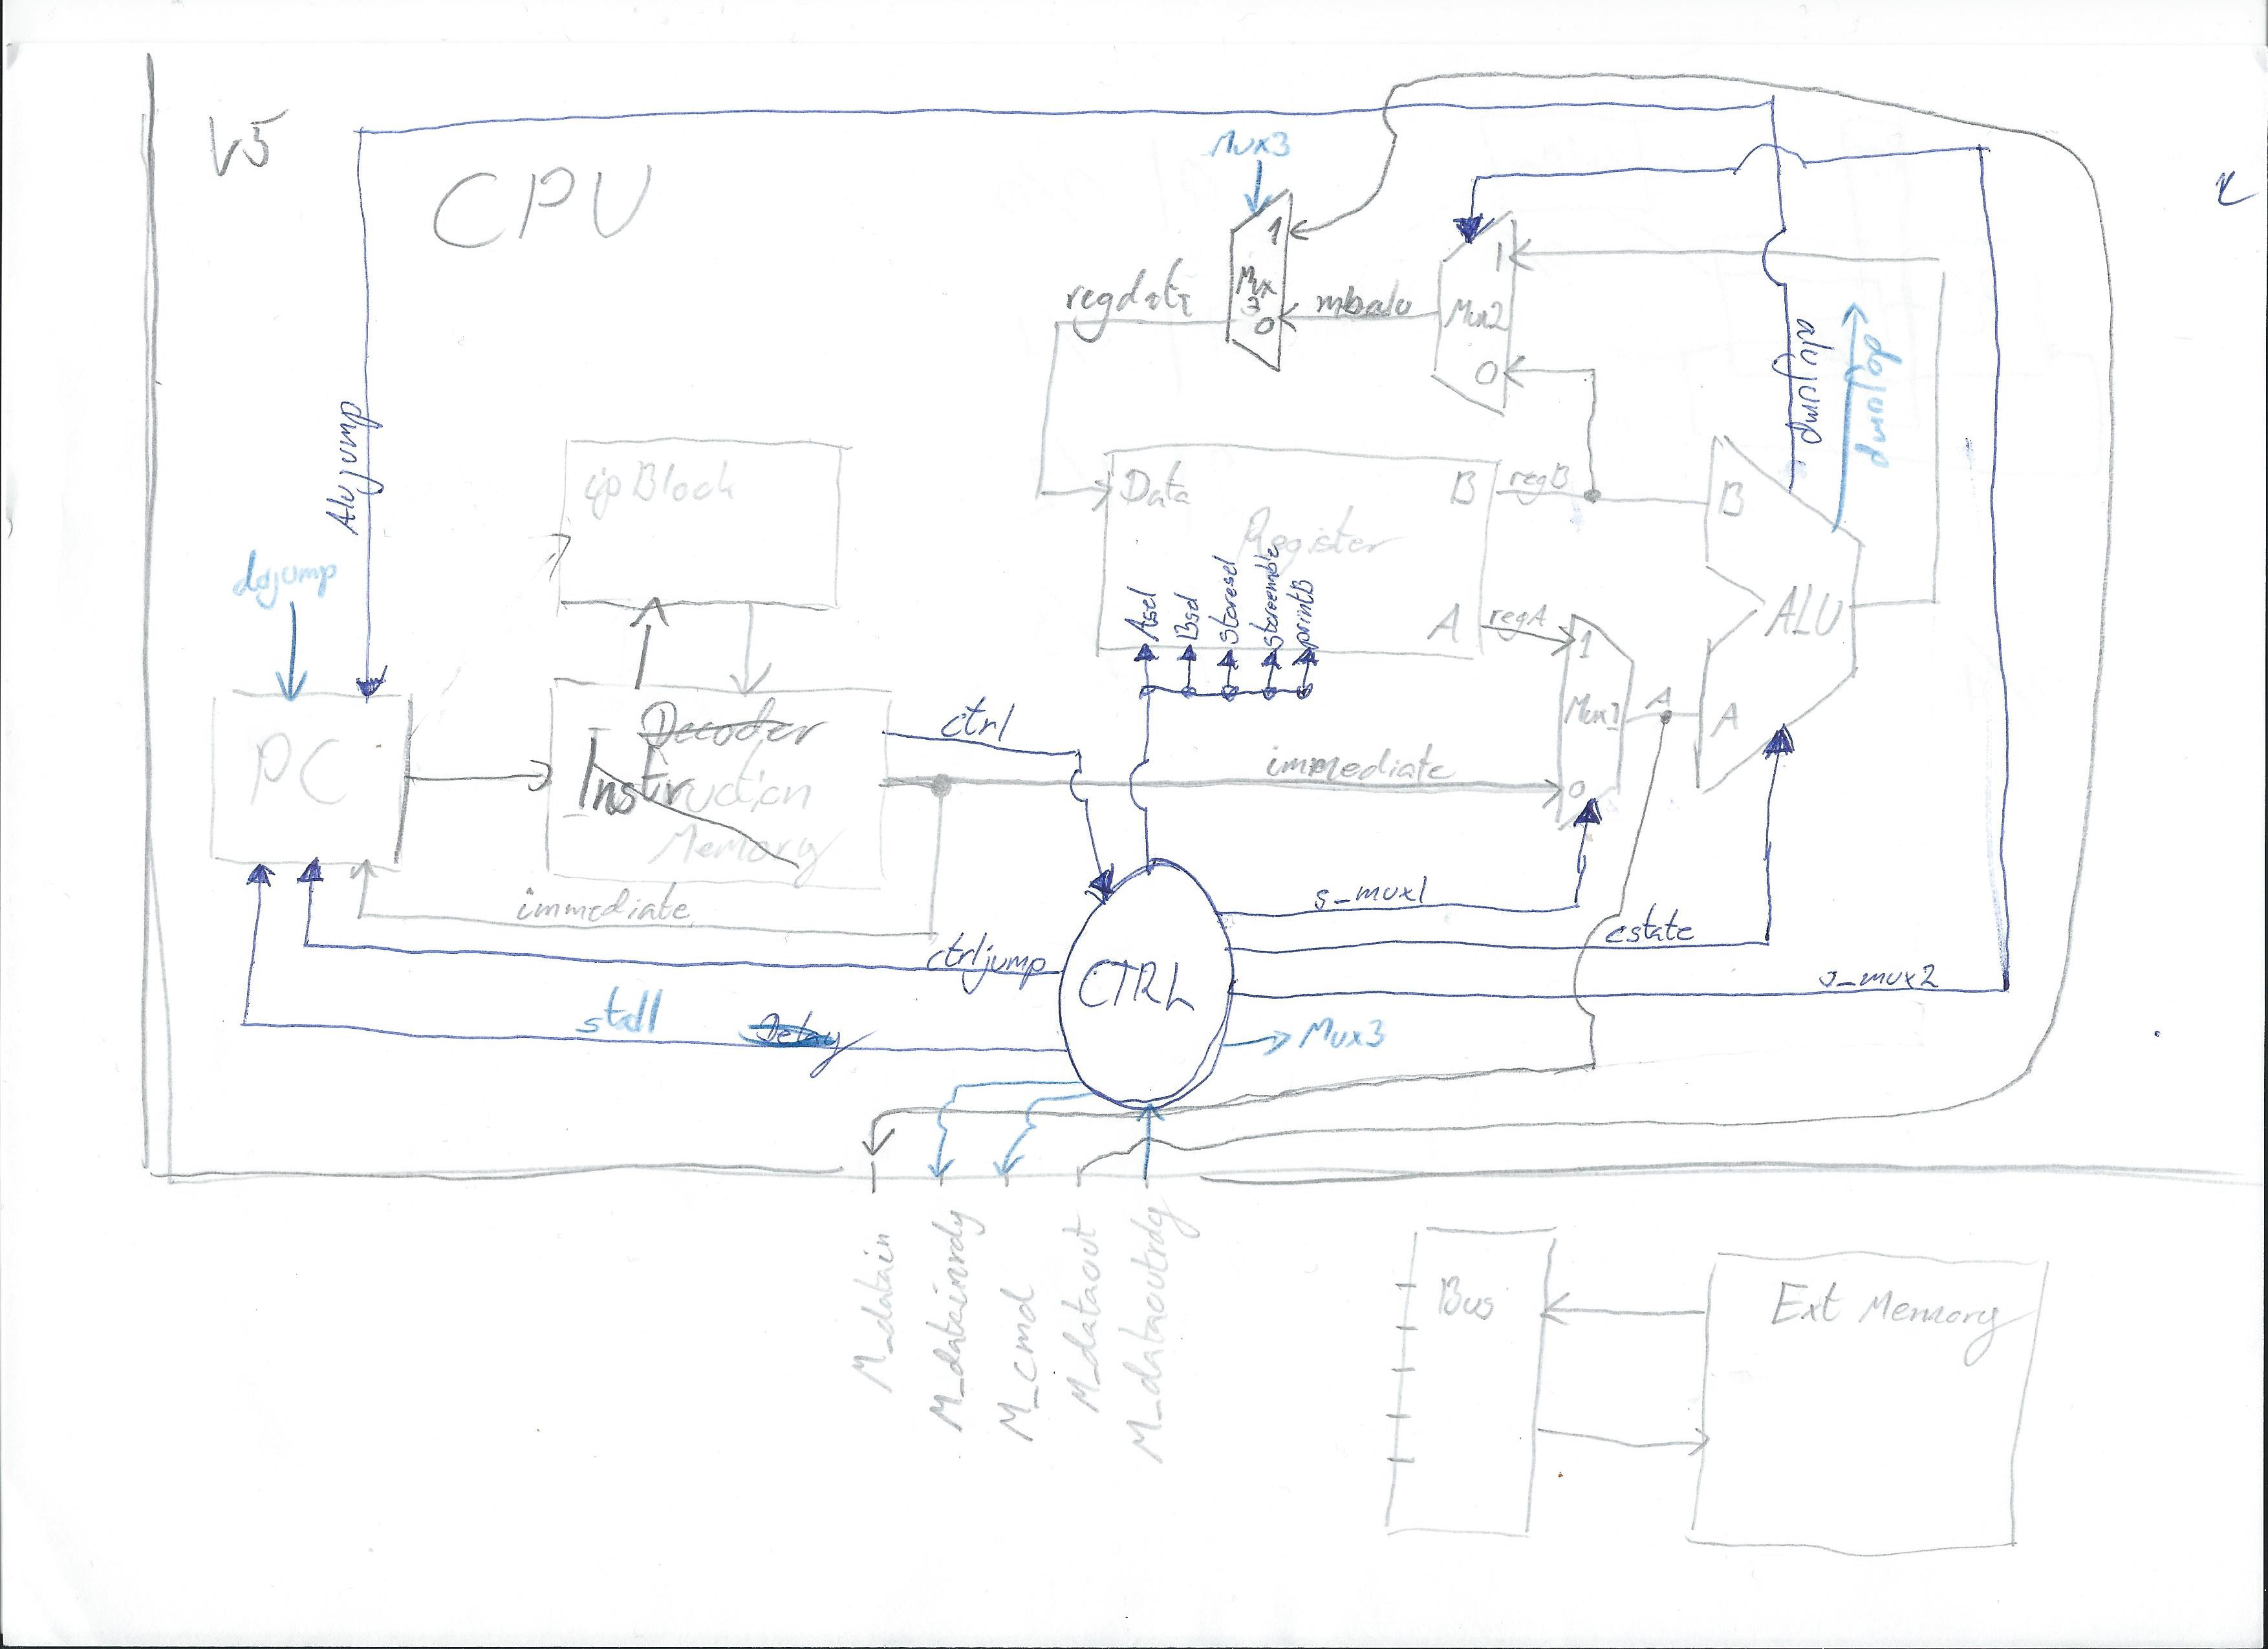
\includegraphics[width=1\textwidth]{Screenshots/Screenshot_DesignDiagram.jpg}
		\caption{The Design diagram of the CPU}
		\label{DesignDiagram}
	\end{figure}
	\\	
	For the sake of clarity the different instructions were implemented through a Finite State Machine with only one state. This allowed for execution of separate Signal Flow Graphs for the individual instructions, grouping their signals together and easing the distinction between control- and data signals. A pure combinatorial implementation could have been used instead but was found to clutter the overview and make it harder to figure out exactly what was going on for each instruction.\\
	As it turned out that the ipblock used for instruction memory contained a register on the inside, there was no direct access to the current address read. Therefore the system needed to stay one command behind all the time. 
	Furthermore, given the fact that the ipblock could only be changed with a 1-clock delay, implementing a jump-signal required support for a built-in stall-signal for the system to wait till the ipblock could return the correct address. This was fixed by adding a stall-signal from the controller and setting it high for each jump-command which would stall for 1 cycle, effectively adding a NOP and letting the ipblock catch up.
	
\subsection{System Integration}
	For attaching the CPU to an actual platform, a premade $Platform.fdl$ was supplied, containing a bus, an external memory as well as a template for a CPU datapath. The CPU template provided 3 output signals and 2 input signals. Communicating with the bus and external memory was then a matter of writing and reading the correct data on the signals at the right time. However, communicating with external devices in this way cannot be done on a single clock-cycle and will generally have to wait for a ready-signal. Therefore the CPU diagram from before needed to be extended to support a wait signal. 
Furthermore, a few registers were added to the CPU datapath to allow for saving the control state while waiting for return signal, as well as maintaining the bus command until it returned.
	When the CPU had been updated and knew how to wait for a signal, a few more modifications were made to the overall diagram to pass data back and forth to the CPU external signals and finally the system was working.
	
\subsection{Critical parts}
	As was stated in the analysis, the critical parts involve three different things to be measured: Speed, size and power.\\
	Speed is measured in clock cycles as well as efficiency per command. For this program there were 11 instructions. 7 of which takes 1 clock cycle to execute (Registers and Arithmetic), 2 that takes 2 cycles (jumps), and the last two that takes 8 and 9 clock cycles, LOAD and STRE respectively. For each data point after the 30'th, the program will carry out these instructions such that in total, each data point requires an estimated 27 clock cycles. Furthermore, the processor had to be able to handle 250 data points per second. With this knowledge, it's possible to calculate the number of clock cycles the processor MUST be able to handle per second, which is $27*250=6750$ clock cycles per second, after the 30'th data sample. This may initially seem like a high amount of cycles, but when compared to the fact that a standard, all-purpose processor like the Core I5 (which is a mid-range processor introduced in 2009 by Intel and used in many computers nowadays) runs at 2.7 GHz for the lowest, which is equivalent to 2.700.000.000 clock cycles per second, 6750 cycles does not seem like much and should be easily accomplished by the processor developed here.\\
	It should be noted here that clock cycles does not have any defined period, and some clock cycles are faster than other (for instance, 1 multiplication followed by a division could take 10ns, whereas 2 additions and an \& might only take 6ns). Therefore, to get a completely accurate view of this, it would be necessary to test how long the program actually takes to calculate these 250 data points, and then subsequently divide this number by 6750 (as this is the amount of clock cycles it should've taken). This would then give an average clock period per cycle.\\
	A guestimate on the optimal clock speed of our processor would therefore be around 15 KHz, which should be more than enough to calculate the necessary 250 data points per second and still have plenty of clock cycles to spare, should some of the clock cycles take drastically longer than others.\\
	\\
	In terms of size, this program has not been optimized for size - first and foremost, the importance was to ensure the program ran correctly and that it ran fast enough to accomplish the necessary 250 data points per second. Many of the data signals have been implemented with excess amount of bits to be certain that the initial product would never run into an overflow. To optimize for size many of these signals could be analysed for maximum values and scaled down to more reasonable width.\\
	\\
	Finally, in terms of power, the main thing to look at would be the number of signals that switches value, also called toggles. Gezel has a built in option to analyse this, and a screenshot of this can be seen below (the full toggle report can be seen here: \ref{toggle_full}):\\
	\begin{figure}[h!]
		\centering
			\includegraphics[width=1\textwidth]{Screenshots/Screenshot_profiling.png}
		\caption{A screenshot of the output of the toggle profiling result.}
		\label{toggle}
	\end{figure}
	
	What can be seen on figure \ref{toggle} is the sum of toggles caused by the different low-level operations. This displays how many evaluations (Evals) and how many toggles there are for each 
	 list of cycles, their evaluations, the number of toggles and the values of all signals, be they 0 or 1. The interesting thing here is to look at the amount of toggles per cycle, as this is what can be optimized. To figure out where to optimize the program in terms of power, the whole simulation is profiled with toggling, the weakest points are identified and evaluated for smarter solutions.\\


\section{Results}
	
%	\begin{figure}[h!]
%		\centering
%			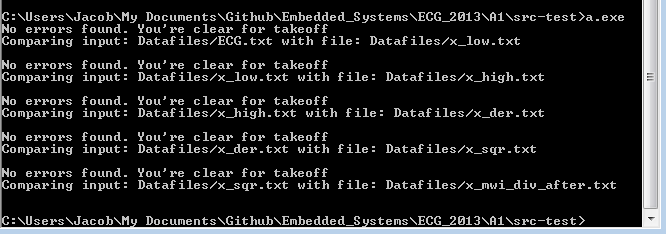
\includegraphics[width=1\textwidth]{Screenshots/tests_filter_result.png}
%		\caption{A screenshot of the output of the tests of the filters.}
%		\label{test_filter_result}
%	\end{figure}

\section{Design}
One of the more important design decisions when designing this processor was how to divide. This is not a simple thing to do in the hardware domain, and as a result, doing the division by 30 could cause problems. To handle this, a python script was created that would determine how to obtain the best approximation, and the end result was an approximation gained by multiplying by 4369 and subsequently bitshifting by 17, both of which are simple operations already implemented in Gezel. By changing the original C-code to perform this approximation instead and approximated output-file was made. This output was then compared to the original output which yielded a difference on 374 out of 10.000 data samples with a maximum error of 1. This was found to be acceptable, as the values the processor operates on are in the several thousands, meaning that the approximation are off by less than 1\textperthousand. Furthermore, it should be noted that the data is already rounded off by the fact that they are integers.\\
\\
Furthermore, it was decided that, rather than make a loop that would run through backwards and gather the 30 data points, the processor would instead simply hold an accumulation of the last 30 values. To this, it would add the next data point and subtract the point that was 30 points old and then subsequently multiply and bitshift - this should give a dramatical increase in calculation speed, as it no longer needs to loop back 30 data points and load all these before it multiplies and bitshifts. The benefit of this is that instead of making 30 additions and 30 divisions, the program need only make one addition, one subtraction and one division, which will increase the speed at which the algorithm runs. For this kind of filter, the output is only valid after it has gathered the initial 30 samples.\\
\\
It was also decided that a new register had to be implemented in the decoder. The value of instVal would be stored in this register, and then read in the following clock cycle. The reason that this was necessary was that, due to the way Gezel is implemented, the signal of instVal would arrive a clock cycle earlier than its corresponding control signal. This workaround is not optimal, but it means that the program works as expected.\\
In the same way as above, another workaround was created around the fact that the ipblock will read an extra line whenever a jump command is sent before actually jumping. The workaround implemented here was to make a NoOPeration (NOP) after each jump, which wastes a cycle but ensures that the program calculates correctly after a jump command.\\
\\

\subsection{Improvements}
To improve on the design, changing the value of the MWI filter to sum over and divide by 32 would make both the implementation, maintenance and all the calculations involved much simpler. Dividing by 32 is a matter of bitshifting right by 5 and no further calculations is necessary. Doing this would not include more additions either, thanks to the way that the summation has been implemented - all that should be changed would be to change the reference of how many steps back the program should go before subtracting. This goes beyond the scope of this report, though.
Another benefit from using 32 instead of 30 would be to simplify implementation of a circular buffer. In assignment 1 a circular buffer was implemented by a struct, a method for incrementing the counter and a method for resetting the counter, when it should loop. Making a circular buffer of 32 values, the counter only needs be 5 bits thus making the reset method redundant as the counter would automatically reset on overflow\\
\\
A further improvement could be to do the addition and the subtraction in one cycle by combining the commands into one accumulator command. This would spare one clock cycle data sample and due to addition and subtraction being simple operations, combining these would probably not extend the critical path of the system. Similarly multiply and bitshift can be combined into a single "divide by 30 approx" command. Even though multiply is a fairly complex operation, in this case it will always multiply by a constant of 4369 which simplifies the operation. Bitshifting on the other hand, is completely free as it can be a case of connecting certain wire-ends on one side to other wire-ends on another. Therefore combining multiply and bitshift into 1 command would probably no extend the critical path either and thus save the system 1 cycle per datasample.\\
\\
The final improvement that this report has been able to identify would be to optimize the signal width; according to the data used in this report, no point is larger than 10.000, which means that no signal needs be larger than 14 bit, and thus could be reduced quite a lot - to take into account, they could be reduced to a bitwidth of about 16 and still be within the limits of the data provided.\\

\section{Conclusion}
It has now been successfully demonstrated that it is possible to implement a dedicated processor for the task of calculating the data of the Mowing Window Integration filter. Furthermore, the critical parts of the processor has been analysed, and the speed of the processor has been determined, along with a way to optimize it in terms of both size and power.
\newpage
\begin{thebibliography}{9}

\bibitem{lamport94}
  Michael Reibel Boesen, Jan Madsen, Linas Kaminskas, Paul Pop, Karsten Juul Frederiksen\\
  \emph{Assignment 2: The ECG processor}\\
  2013.\\

\bibitem{Gezel}
  \emph{Lecture7: Finite state machine with Datapath}\\
  Fall, 2007.\\

\bibitem{GezelBasicSyntax}
  \emph{GEZEL Basic Syntax}\\
  
\bibitem{ClockSpeeds}
  \emph{http://smallbusiness.chron.com/ghz-mean-computer-processor-66857.html}
  Used to explain clock speeds of a processor
  
\bibitem{CoreI5}
  \emph{http://www.intel.com/content/www/us/en/processors/core/core-i5-processor.html}
  Used to determine clock speeds of Core I5
\end{thebibliography}
	
\newpage	
	\begin{Large}
		\textbf{Appendix}
	\end{Large}
	\appendix

\section{Who wrote what}
Jacob Gjerstrup, s113440 wrote: Introduction, Analysis (Problem 1, 2 and 5), Implementation (Processor, Instruction set, Critical Parts), Design\\
Jakob Welner, s124305 wrote: Abstract, Analysis (Problem 3+4), Implementation (Implementation of the CPU, System Integration), Design (Improvements section), Conclusion\\

\section{Sourcecode}

\subsection{Source code for the Processer modules}
	\subsubsection{Counter}
		\lstinputlisting[language=C]{Code/Proc_Mods/counter.fdl}	
	\subsubsection{Adder with testbench}
		\lstinputlisting[language=C]{Code/Proc_Mods/adder.fdl}	
	\subsubsection{Multiplexer}
		\lstinputlisting[language=C]{Code/Proc_Mods/mux.fdl}	
	\subsubsection{Arithmetic Logic Unit (ALU)}
		\lstinputlisting[language=C]{Code/Proc_Mods/ALU.fdl}
	\subsubsection{ALU with flags}
		\lstinputlisting[language=C]{Code/Proc_Mods/ALU_withFlags.fdl}	
	\subsubsection{Register}
		\lstinputlisting[language=C]{Code/Proc_Mods/register.fdl}	
	\subsubsection{Instruction Memory}
		\lstinputlisting[language=C]{Code/Proc_Mods/memory.fdl}	
\subsection{Instruction set}
	\lstinputlisting[language=C]{Code/assembly_mwint.asm}	
\subsection{CPU}
	\lstinputlisting[language=C]{Code/CPU.fdl}
\subsection{Profiling}
	\label{toggle_full}	
	\lstinputlisting[language=C]{Code/toggle_output.txt}

\subsection{Python scripts}
	The script to find the division approximation:
	\lstinputlisting[language=Python]{Code/div30Approx.py}
	
	The script to make the assembly OP-codes:
		\lstinputlisting[language=Python]{Code/assembler.py}
\end{document}